\begin{frame}{训练过程}

    \begin{figure}
        \centering
        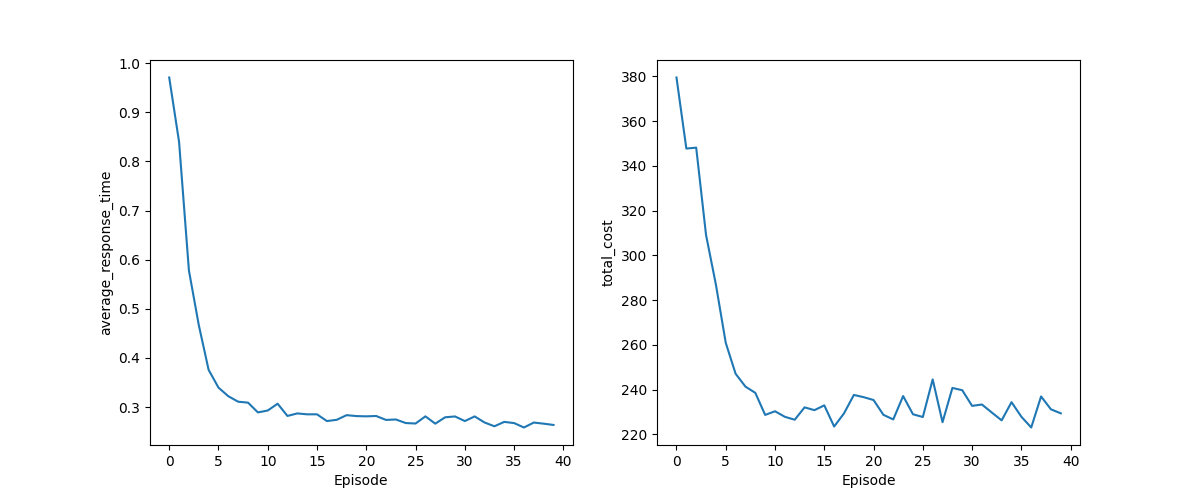
\includegraphics[height=0.7\textheight]{pics/training_track.png}
        \caption{训练过程中任务平均响应时间与价格的变化}
    \end{figure}

\end{frame}

\begin{frame}{DQN 与 Baseline 的对比}{应对不同的任务到达速度}

    \begin{columns}

        \column{0.5\textwidth}

        \begin{figure}
            \centering
            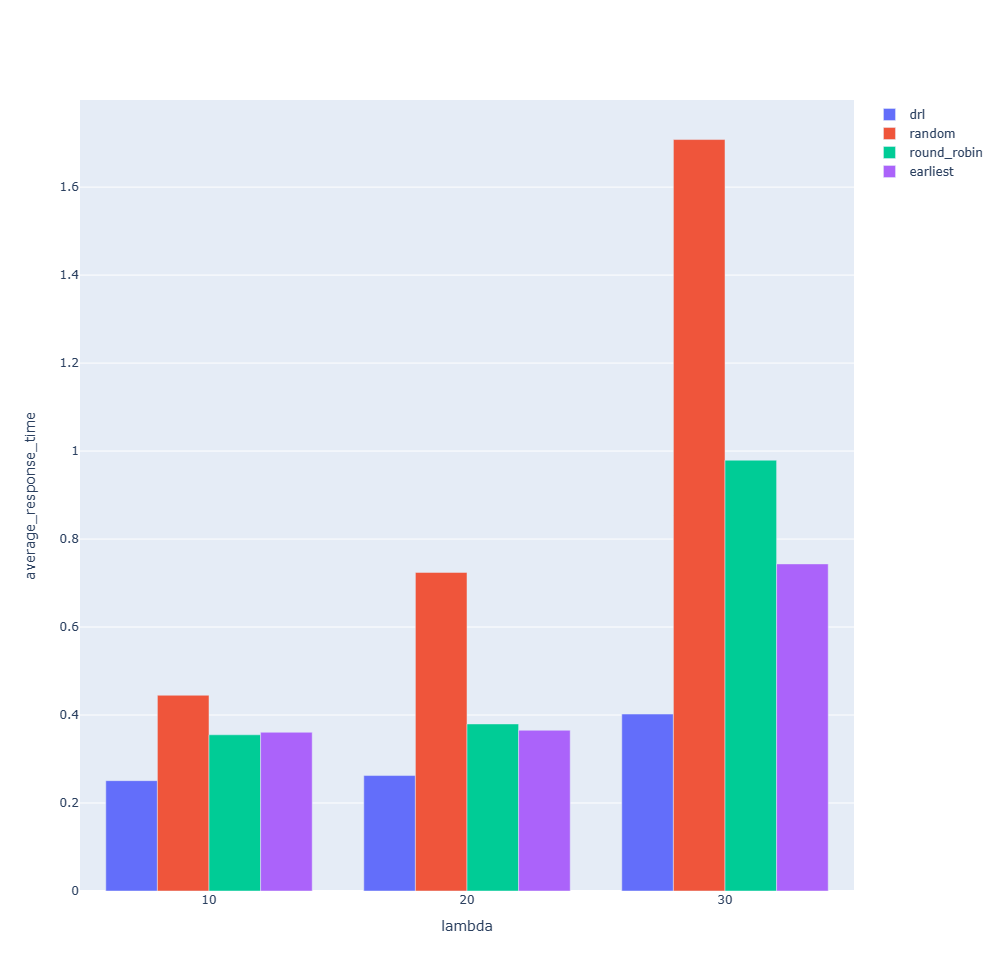
\includegraphics[width=0.9\textwidth]{pics/vary_lambda_resp.png}
        \end{figure}

        \column{0.5\textwidth}

        \begin{figure}
            \centering
            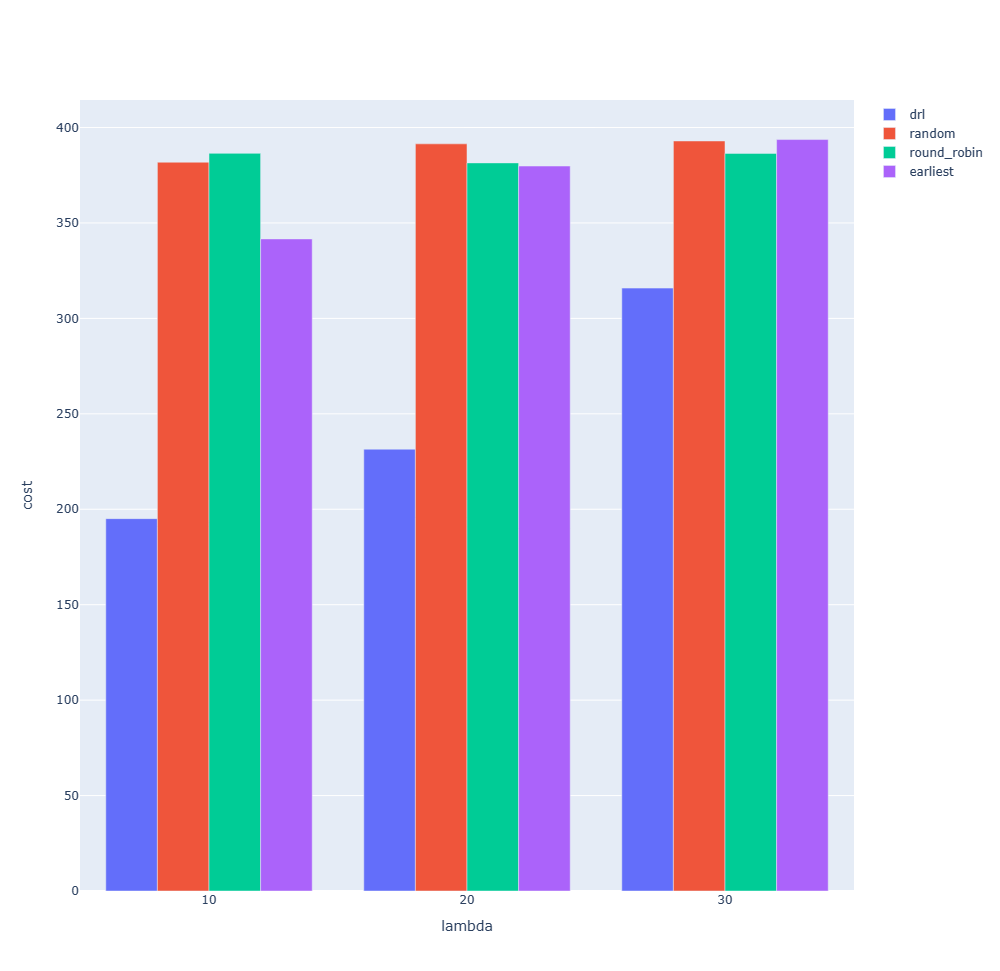
\includegraphics[width=0.9\textwidth]{pics/vary_lambda_cost.png}
        \end{figure}

    \end{columns}

\end{frame}

\begin{frame}{DQN 与 Baseline 的对比}{应对不同的任务类型比例}

    \begin{columns}

        \column{0.5\textwidth}

        \begin{figure}
            \centering
            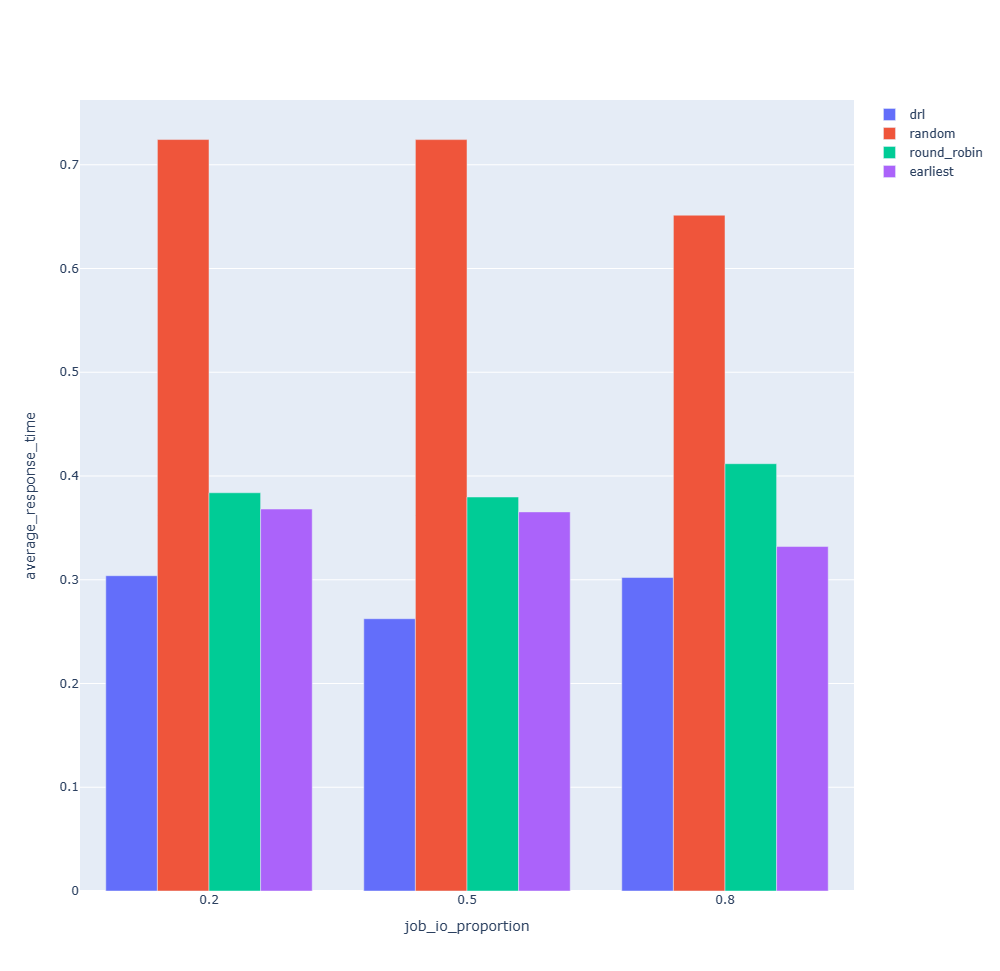
\includegraphics[width=0.9\textwidth]{pics/vary_job_resp.png}
        \end{figure}

        \column{0.5\textwidth}

        \begin{figure}
            \centering
            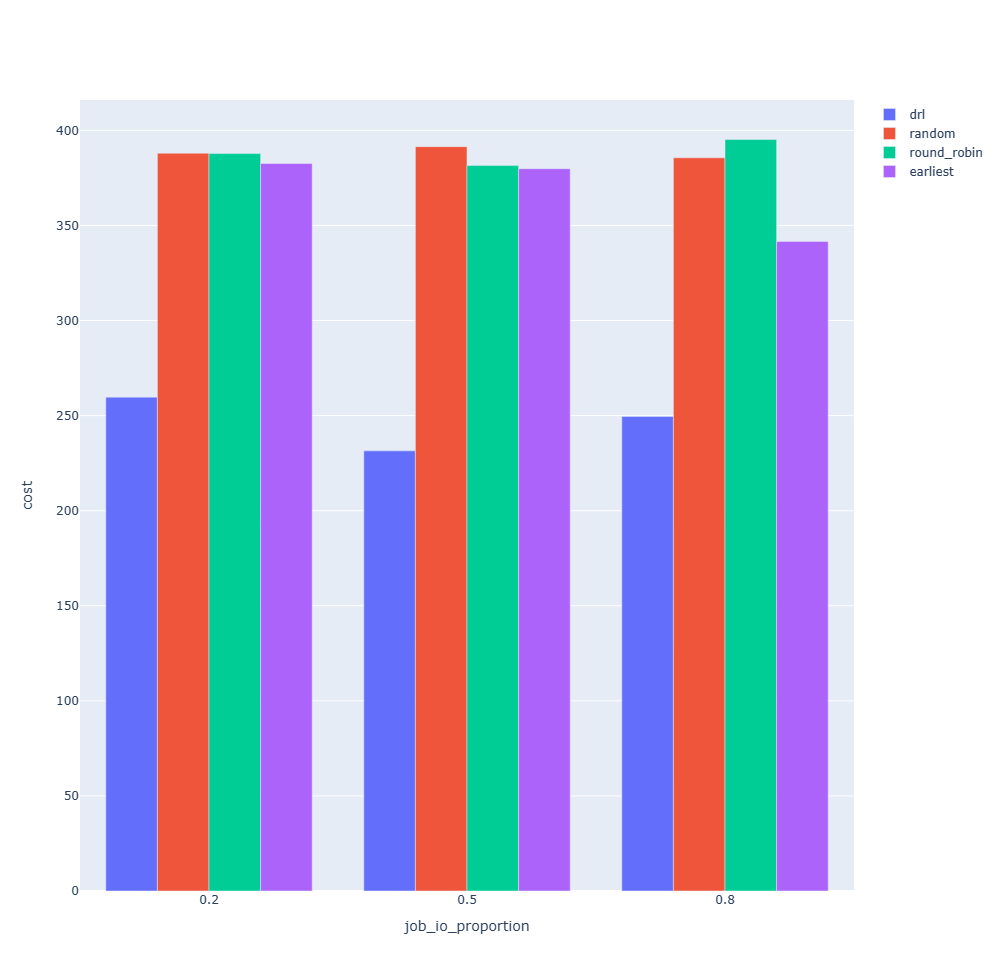
\includegraphics[width=0.9\textwidth]{pics/vary_job_cost.png}
        \end{figure}

    \end{columns}

\end{frame}

\begin{frame}{DQN 与 Baseline 的对比}{应对不同的虚拟机类型比例}

    \begin{columns}

        \column{0.5\textwidth}

        \begin{figure}
            \centering
            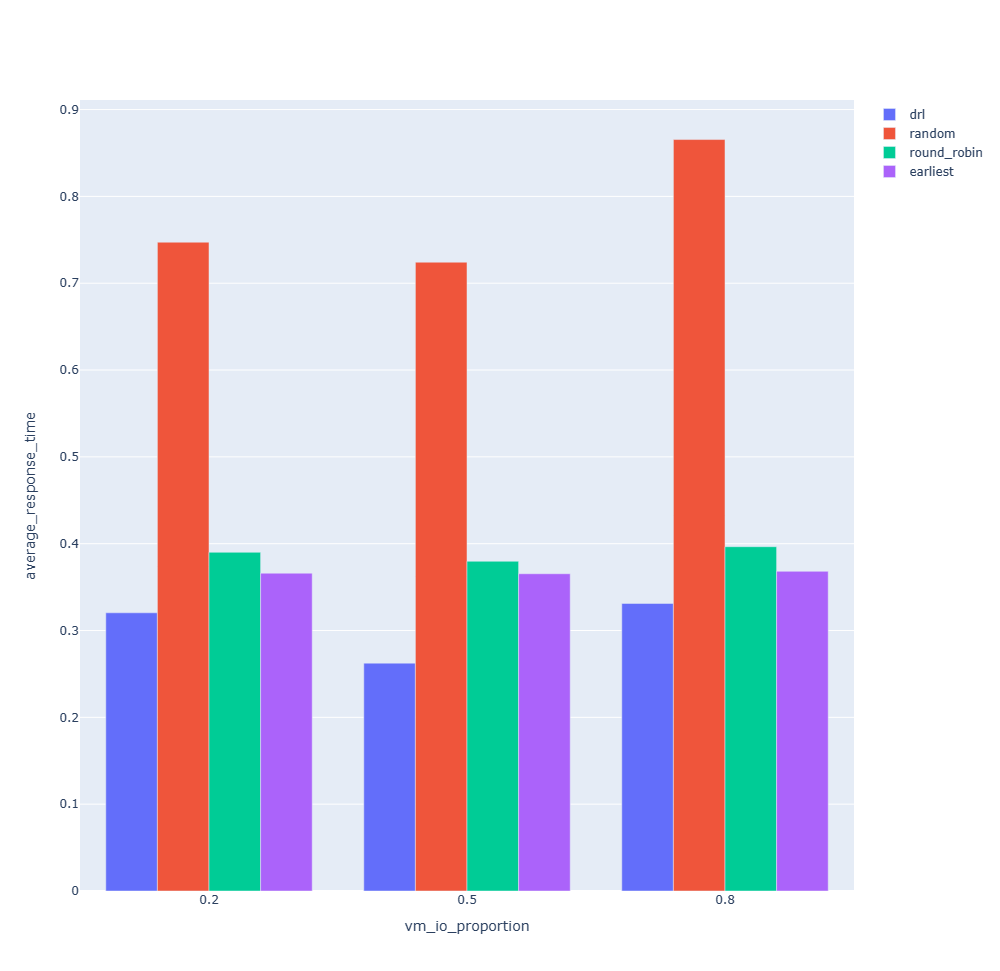
\includegraphics[width=0.9\textwidth]{pics/vary_vm_resp.png}
        \end{figure}

        \column{0.5\textwidth}

        \begin{figure}
            \centering
            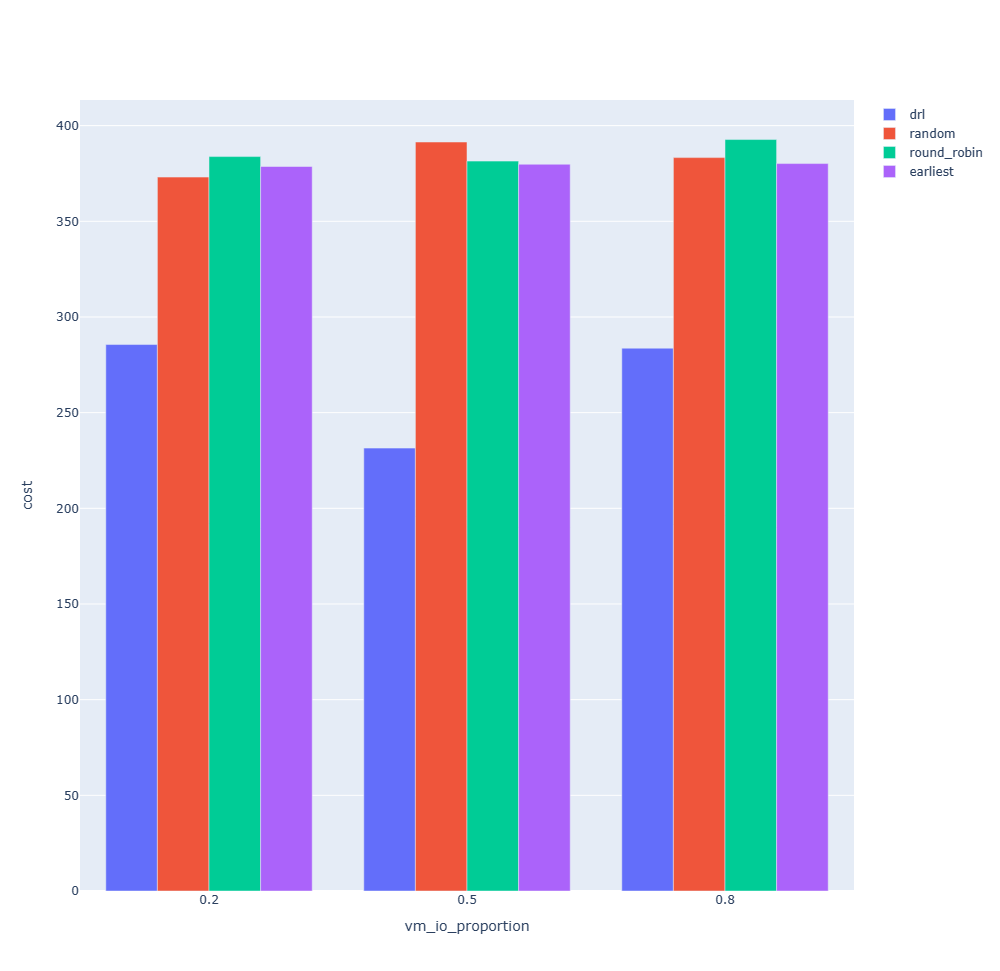
\includegraphics[width=0.9\textwidth]{pics/vary_vm_cost.png}
        \end{figure}

    \end{columns}

\end{frame}
